%----------------------------------------------------------------------------------------
%    PACKAGES AND THEMES
%----------------------------------------------------------------------------------------

\documentclass[aspectratio=169,xcolor=dvipsnames]{beamer}
\usetheme{SimplePlus}

\usepackage{hyperref}
\usepackage{graphicx} % Allows including images
\usepackage{booktabs} % Allows the use of \toprule, \midrule and \bottomrule in tables
\usepackage{bbm}

%----------------------------------------------------------------------------------------
%    TITLE PAGE
%----------------------------------------------------------------------------------------

\title{A Survey of NL2SQL with Large Language Models: Where are we, and where are we going?}
% \subtitle{Subtitle}

\author{Speaker: Jiahao He}

\institute
{
    School of Information \\
    Renmin University of China % Your institution for the title page
}
\date{\today} % Date, can be changed to a custom date

%----------------------------------------------------------------------------------------
%    PRESENTATION SLIDES
%----------------------------------------------------------------------------------------

\begin{document}

\begin{frame}
    % Print the title page as the first slide
    \titlepage
\end{frame}


\begin{frame}{Motivating Example}
    \textbf{NL query: }\textit{Find the \textcolor{orange}{names} of all \textcolor{red}{customers} who checked out \textcolor{red}{books} on exactly 3 different \textcolor{orange}{genres} on \textcolor{blue}{Labor Day in 2023}.}

    \textbf{Database:}

    \begin{columns}[T]
        \begin{column}{.3\textwidth}
            \begin{table}
                \begin{tabular}{l l l}
                    \toprule
                    \multicolumn{3}{l}{\textcolor{red}{Customer}} \\
                    \midrule
                    CustomerId         & \textcolor{orange}{Name}          & ...\\
                    \bottomrule
                \end{tabular}
            \end{table}
        \end{column}

        \begin{column}{.6\textwidth}
            \begin{table}
                \begin{tabular}{l l l l l}
                    \toprule
                    \multicolumn{5}{l}{\textcolor{red}{Book}} \\
                    \midrule
                    BookId         & Title          &\textcolor{orange}{LiteralGenres} & \textcolor{orange}{SubjectGenres} & ...\\
                    \bottomrule
                \end{tabular}
            \end{table}
        \end{column}
    \end{columns}

    \begin{table}
        \begin{tabular}{l l l l}
            \toprule
            \multicolumn{4}{l}{BookOrder} \\
            \midrule
            CustomerID         & BookID          &\textcolor{purple}{OrderDate} & ...\\
            \bottomrule
        \end{tabular}
    \end{table}
    Additional Information: Note that \textcolor{purple}{Labor Day stands for May 1\textsuperscript{st}}.
\end{frame}

\begin{frame}{Motivating Example}
    \begin{enumerate}
        \item Find key components in NL: \textcolor{red}{entities}, \textcolor{orange}{attributes}, \textcolor{blue}{temporal information}, specific conditions\dots
        \item Find relevant tables, columns and, cell values in DB: \textcolor{red}{Customer}, \textcolor{red}{Book}, \textcolor{red}{BookOrder}, \textcolor{orange}{Name}, \textcolor{orange}{LiteralGenres}, \textcolor{orange}{SubjectGenres}\dots
        \item Writing SQL base on NL and DB understanding:
    \end{enumerate}
    \begin{columns}[T]
        \begin{column}{0.45\textwidth}
            \texttt{SELECT FROM \textcolor{red}{Customer}} 
            
            \texttt{NATURAL JOIN \textcolor{red}{BookOrder}}

            \texttt{NATURAL JOIN \textcolor{red}{Book}}
            
            \texttt{WHERE \textcolor{orange}{OrderDate}=\textcolor{blue}{'2023-05-01'}}
            
            \texttt{GROUP BY \textcolor{orange}{CustomerId}} 
            
            \texttt{HAVING COUNT(DISTINCT \textcolor{orange}{LiteralGenre})=3}
        \end{column}

        \begin{column}{0.45\textwidth}
            \texttt{SELECT FROM \textcolor{red}{Customer}}

            \texttt{WHERE \textcolor{orange}{CustomerId} = (SELECT CustomerId}
            
            \texttt{FROM \textcolor{red}{BookOrder}} 
            
            \texttt{NATURAL JOIN \textcolor{red}{Book}}  
            
            \texttt{WHERE \textcolor{orange}{OrderDate}= \textcolor{blue}{'2023-05-01'}}
            
            \texttt{GROUP BY \textcolor{orange}{CustomerId}}  
            
            \texttt{HAVING COUNT(DISTINCT \textcolor{orange}{SubjectGenre})=3)}
        \end{column}
    \end{columns}
\end{frame}

\begin{frame}{Chanllenges and Solutions}
    \begin{columns}[T]
        \begin{column}{0.45\textwidth}
            \begin{itemize}
                \item[C1:]\textbf{Uncertain natural language query}: lexical and syntactic ambiguity\dots
                \item[C2:]\textbf{Complex database and dirty content}: complex relations, ambiguity attributes\dots
                \item[C3:]\textbf{NL2SQL translation}: multiple possible queries\dots
                \item[C4:]\textbf{technical challenges in developing NL2SQL solutions}: efficiency, reliability\dots
            \end{itemize}
        \end{column}
        \begin{column}{0.45\textwidth}
            \begin{figure}
                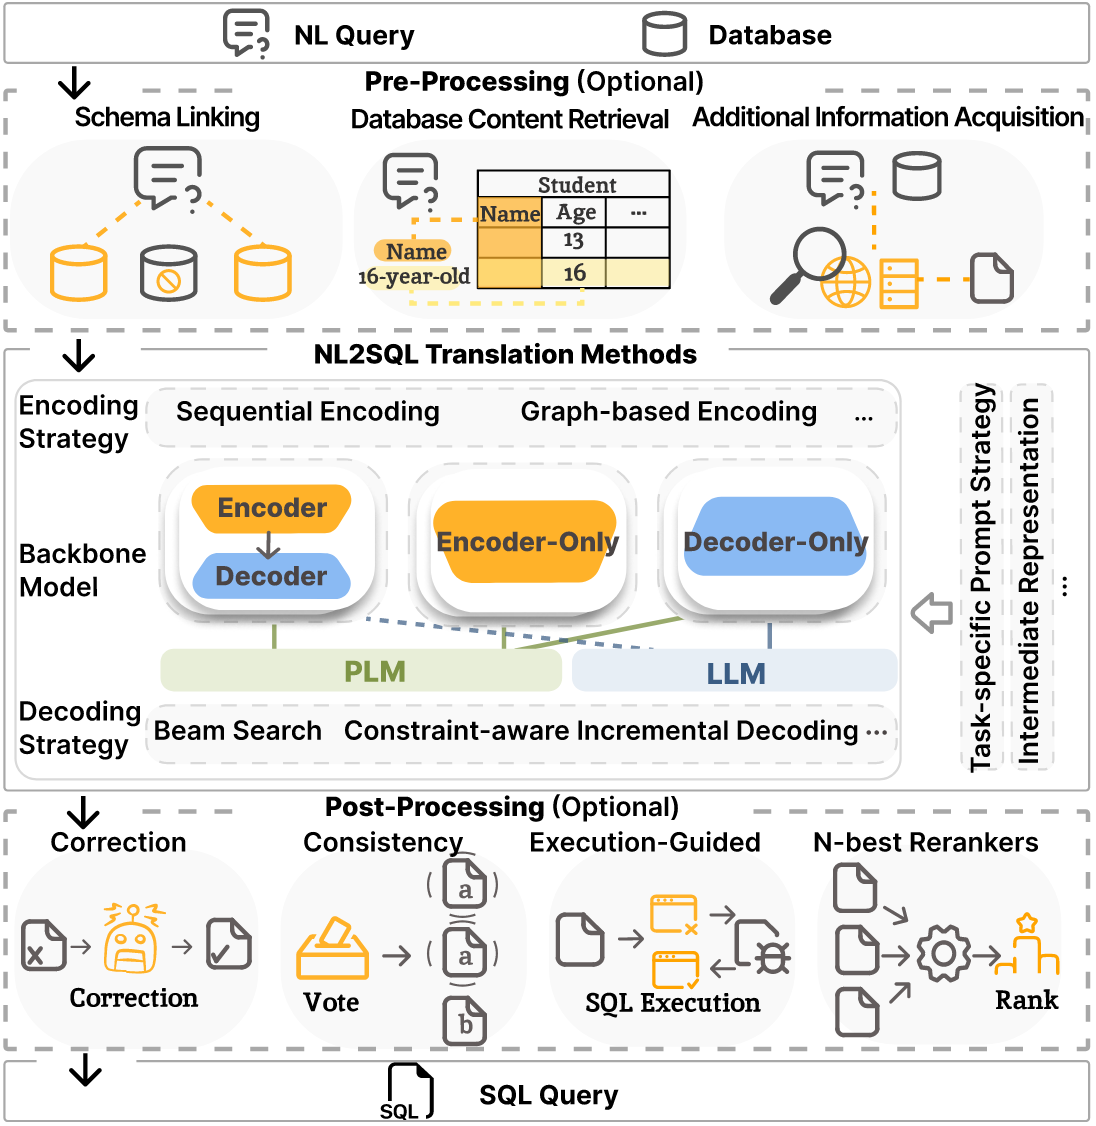
\includegraphics[width=\linewidth]{assets/overview.png}
            \end{figure}
        \end{column}
    \end{columns}
\end{frame}

\begin{frame}{Preprocessing Strategies for NL2SQL}
    \textit{A. Schema Linking}
    \begin{itemize}
        \item String Matching-based: Identifies matches when candidates are identical or when one is a substring of the other. -\alert{struggle with synonyms and vocabulary variations}.
        \item Neural Network-based: Use neural networks to learn the relationship between the NL and the DB schema. -\alert{struggle to generalize across databases}.
        \item In-Context Learning: Utilizes LLMs’ ability to understand complex language patterns and relationships within data schemas. -\alert{computationally expensive}.
        \begin{example}
            Given the database schema and question, perform the following actions:

            1 - Rank all the table base on the possibiliy of being used in the SQL according to the question from the most relevant to the least relevant. Table or its columns that matches more with the question's words is highly relevant and must be placed ahead.

            \dots
        \end{example}
    \end{itemize}
\end{frame}

\begin{frame}{Preprocessing Strategies for NL2SQL}
    \textit{B. Database Content Retrieval}: extracting cell values for specific SQL clauses
    \begin{itemize}
        \item String Matching-based: Simliar with schema linking.-\alert{synonyms and computationally expensive}
        \item Neural Network-based: Capture complex data and semantic features through layers of nonlinear transformations, helping to resolve synonym issues -\alert{ambiguous NL}.
        \item Index-based: Enabling faster access to relevant cell values. -\alert{frequent changes}.
        \begin{example}
            NL: "Show me the names of all employees in the \alert{Sales} department."

            SQL: SELECT Employees.Name  

            FROM Employees  

            JOIN Departments ON Employees.DepartmentID = Departments.DepartmentID  

            WHERE Departments.DepartmentName = '\alert{Sales}';
        \end{example}
    \end{itemize}
\end{frame}

\begin{frame}{Preprocessing Strategies for NL2SQL}
    \textit{C. Additional Information Acquisition}: fetch additional information for the translation.
    \begin{itemize}
        \item Sample-based: Use few-shot examples from extensive domain knowledge
        
        \item Retrieval-based: Retrieval similar information.
        \begin{example}
            NL: \textit{Find the \textcolor{orange}{names} of all \textcolor{red}{customers} who checked out \textcolor{red}{books} on exactly 3 different \textcolor{orange}{genres} on \textcolor{blue}{Labor Day in 2023}.}

            Additional Information: Note that \textcolor{purple}{Labor Day stands for May 1\textsuperscript{st}} in China and \textcolor{purple}{September 4\textsuperscript{th}} in the US.
        \end{example}
    \end{itemize}
\end{frame}

\begin{frame}{NL2SQL Translation Methods}
    \textit{A. Encoding Strategy}
\end{frame}

\begin{frame}{NL2SQL Translation Methods}
    \textit{B. Decoding Strategy}
\end{frame}

\begin{frame}{NL2SQL Translation Methods}
    \textit{C. Task-specific Prompt Strategy}
\end{frame}

\begin{frame}{NL2SQL Translation Methods}
    \textit{D. Intermediate Representation for NL2SQL Translation}
\end{frame}

\begin{frame}{Postprocessing Strategies for NL2SQL}
    \textit{A. SQL Correction Strategies}: Mainly focus on correcting syntax errors in the generated SQL queries.

    \textit{B. Output Consistency}: Ensure that the generated SQL query is consistent with the NL query.

    \textit{C. Execution Guided Strategies}: Refine SQL based on execution results, ensuring the query retrieves data correctly.

    \textit{D. N-best Reranker Strategies}: Reorder the top-N model outputs, often leveraging a larger model (BERT-based reranker) or additional knowledge sources.
\end{frame}

%------------------------------------------------

\begin{frame}{NL2SQL Benchmarks}
    \begin{figure}
        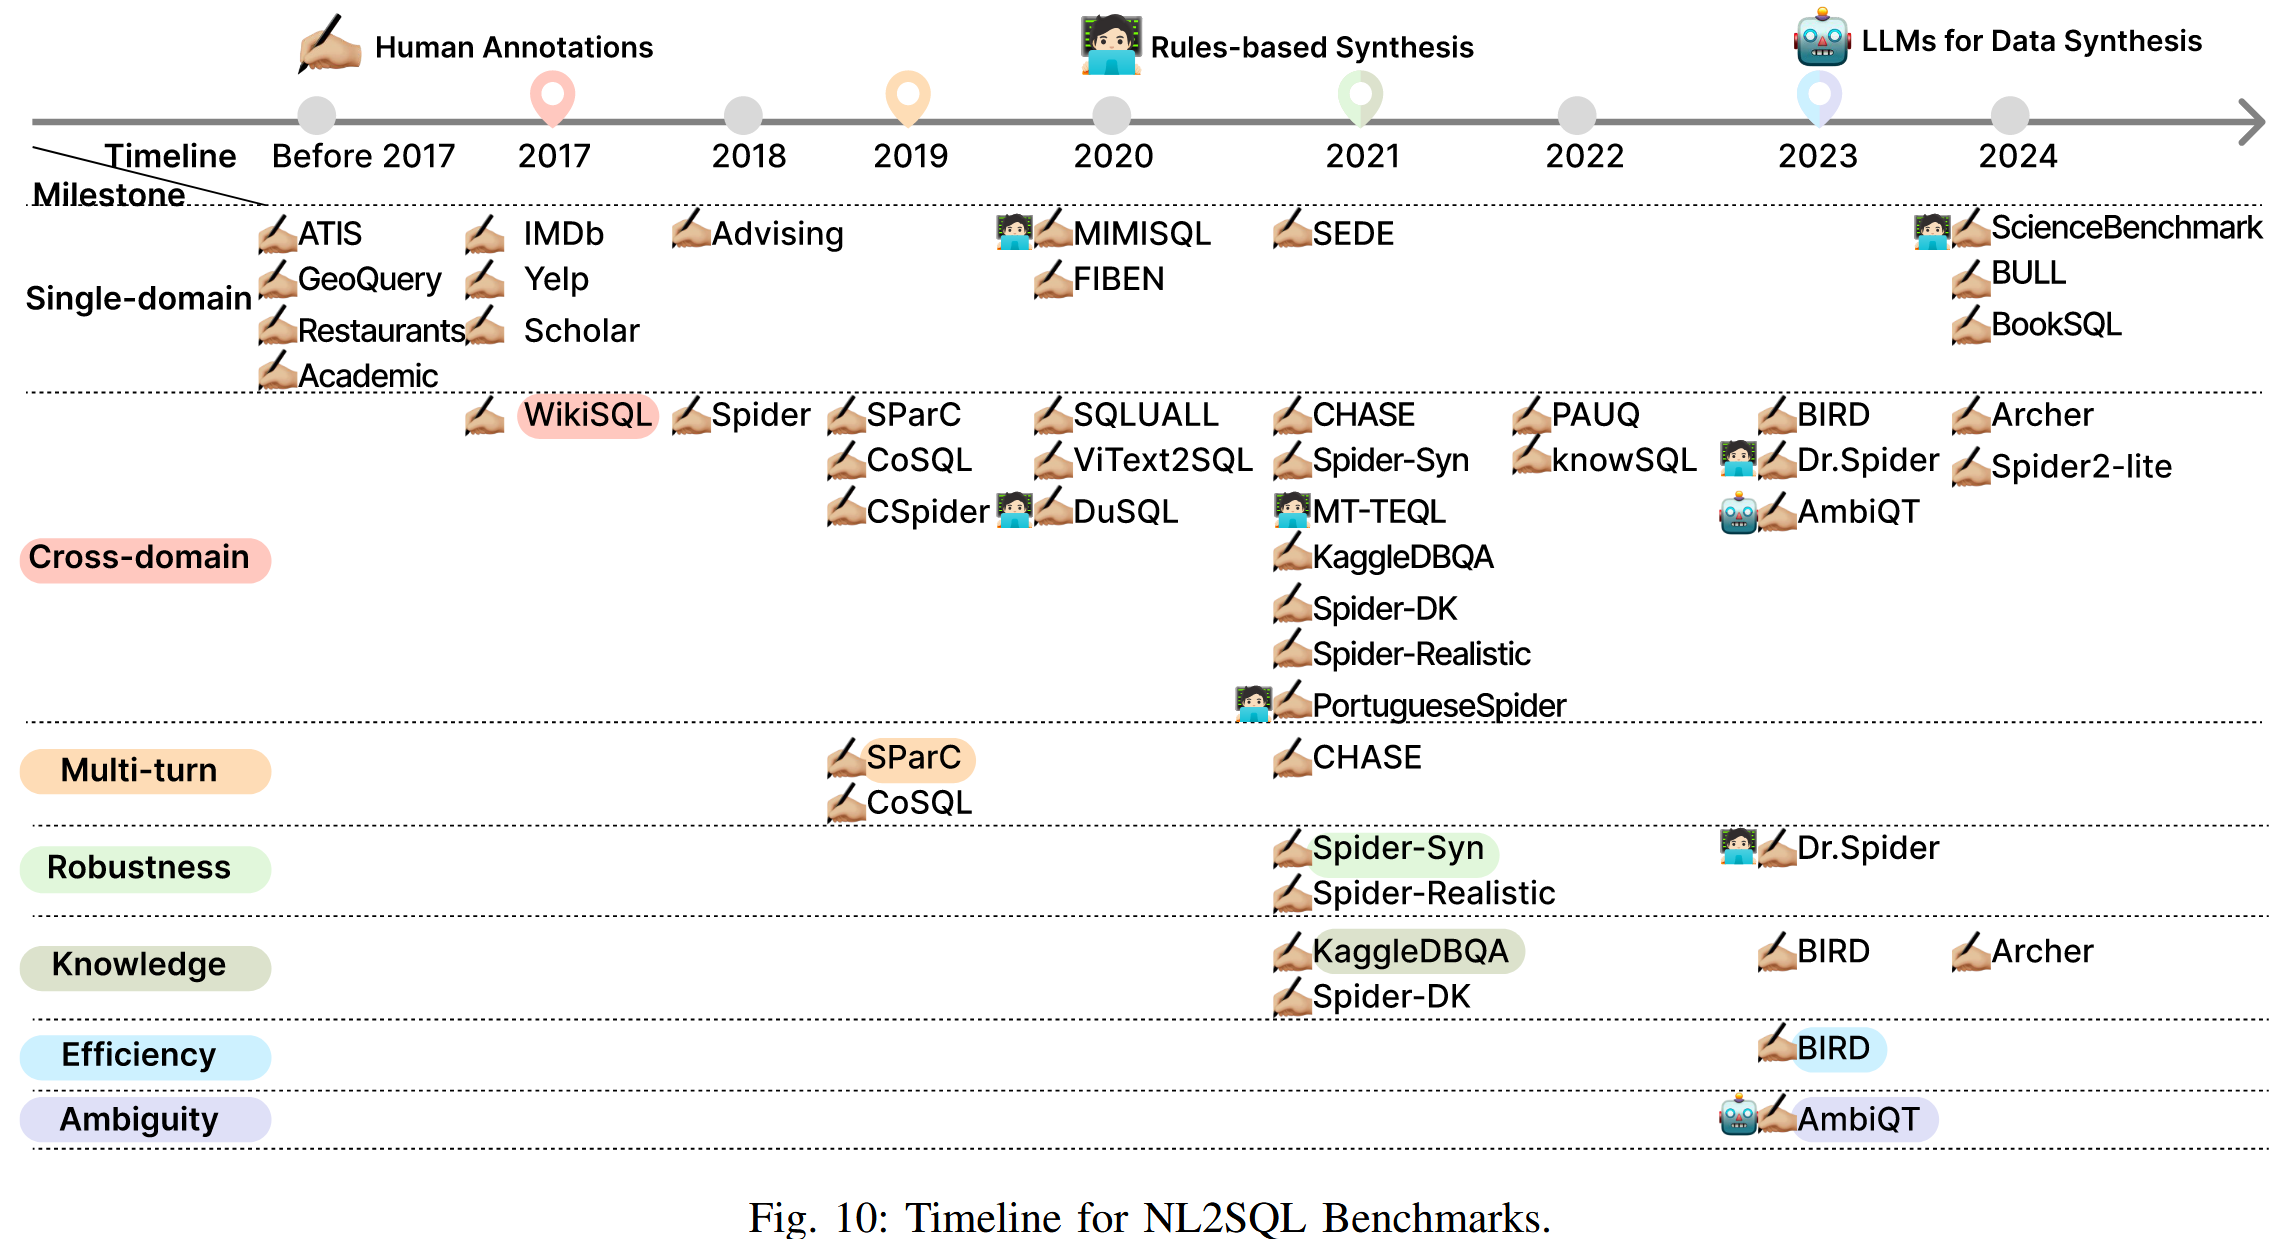
\includegraphics[width=\linewidth]{assets/benchmarks.png}
    \end{figure}
\end{frame}

%------------------------------------------------

\begin{frame}{Evaluation and Error Analysis}
    \textbf{Metrics: }
    \begin{itemize}
        \item \textit{Execution Accuracy(EX):} $EX=\sum_{i=1}^N \mathbbm{1}(V_i=\widehat{V}_i) / N$, $\mathbbm{1}(\cdot)=1$ when $\cdot$ is true, and $0$ otherwise.
        \item \textit{String-Match Acurracy(SM):} $SM=\sum_{i=1}^N \mathbbm{1}(Y_i=\widehat{Y}_i) / N$.
        \item \textit{Component-Match Acurracy(CM):} $CM^C=\sum_{i=1}^N \mathbbm{1}(Y_i^C=\widehat{Y}_i^C) / N$.
        \item \textit{Exact-Match Accuracy(EM):}$EM=\sum_{i=1}^N \mathbbm{1}(\land_{C_k\in \mathbbm{C}} Y_i^{C_k}=\widehat{Y}_i^{C_k}) / N$
        \item \textit{Valid Efficiency Score(VES):}
        \[
            VES=\frac{1}{N}\sum_{i=1}^N \mathbbm{1}(V_i=\widehat{V}_i)\cdot \mathbf{R}(Y_i, \widehat{Y_i}),\quad \mathbf{R}(Y_i, \widehat{Y_i}) =\sqrt{\mathbf{E}(Y_i)/\mathbf{E}(\widehat{Y_i})}
        \]
        \item \textit{Query Variance Testing(QVT):}
        \[
            QVT=\frac{1}{N}\sum_{i=1}^N \left(\frac{\sum_{j=1}^{m_i}\mathbbm{1}\left(\mathcal{F} (Q_{ij})=Y_i\right)}{m_i}\right)
        \]
    \end{itemize}
\end{frame}

\begin{frame}{Evaluation and Error Analysis}
    Evaluation toolkits: MT-TEQL, NL2SQL360\dots

    Error analysis taxonomy:
    \begin{enumerate}
        \item \textit{Error Location}: identify specific SQL components where errors occur, such as the \texttt{SELECT} or \texttt{WHERE} clause.
        \item \textit{Cause of Error}: focus on the underlying reasons for the error.
    \end{enumerate}
    \begin{figure}
        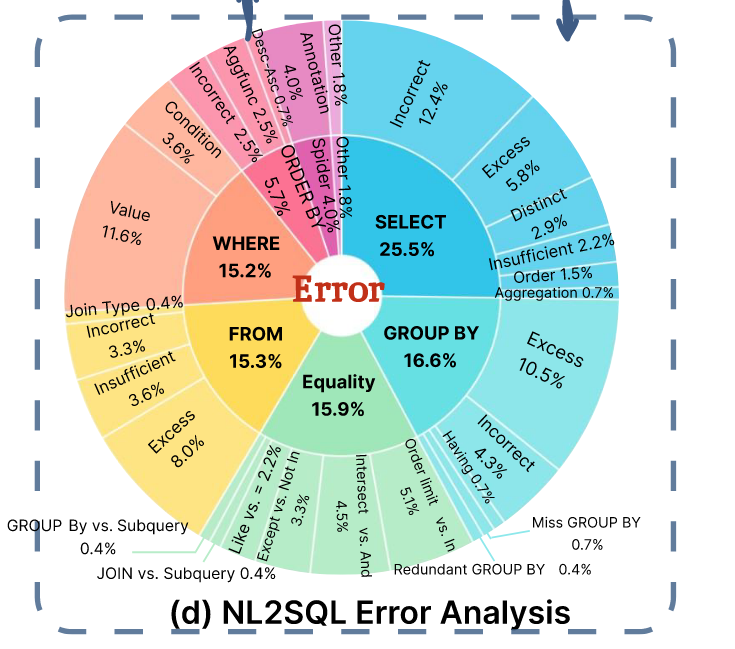
\includegraphics[width=.35\linewidth]{assets/error.png}
    \end{figure}
\end{frame}

%------------------------------------------------

\begin{frame}{Practical Guidance for NL2SQL Solutions}
    \begin{figure}
        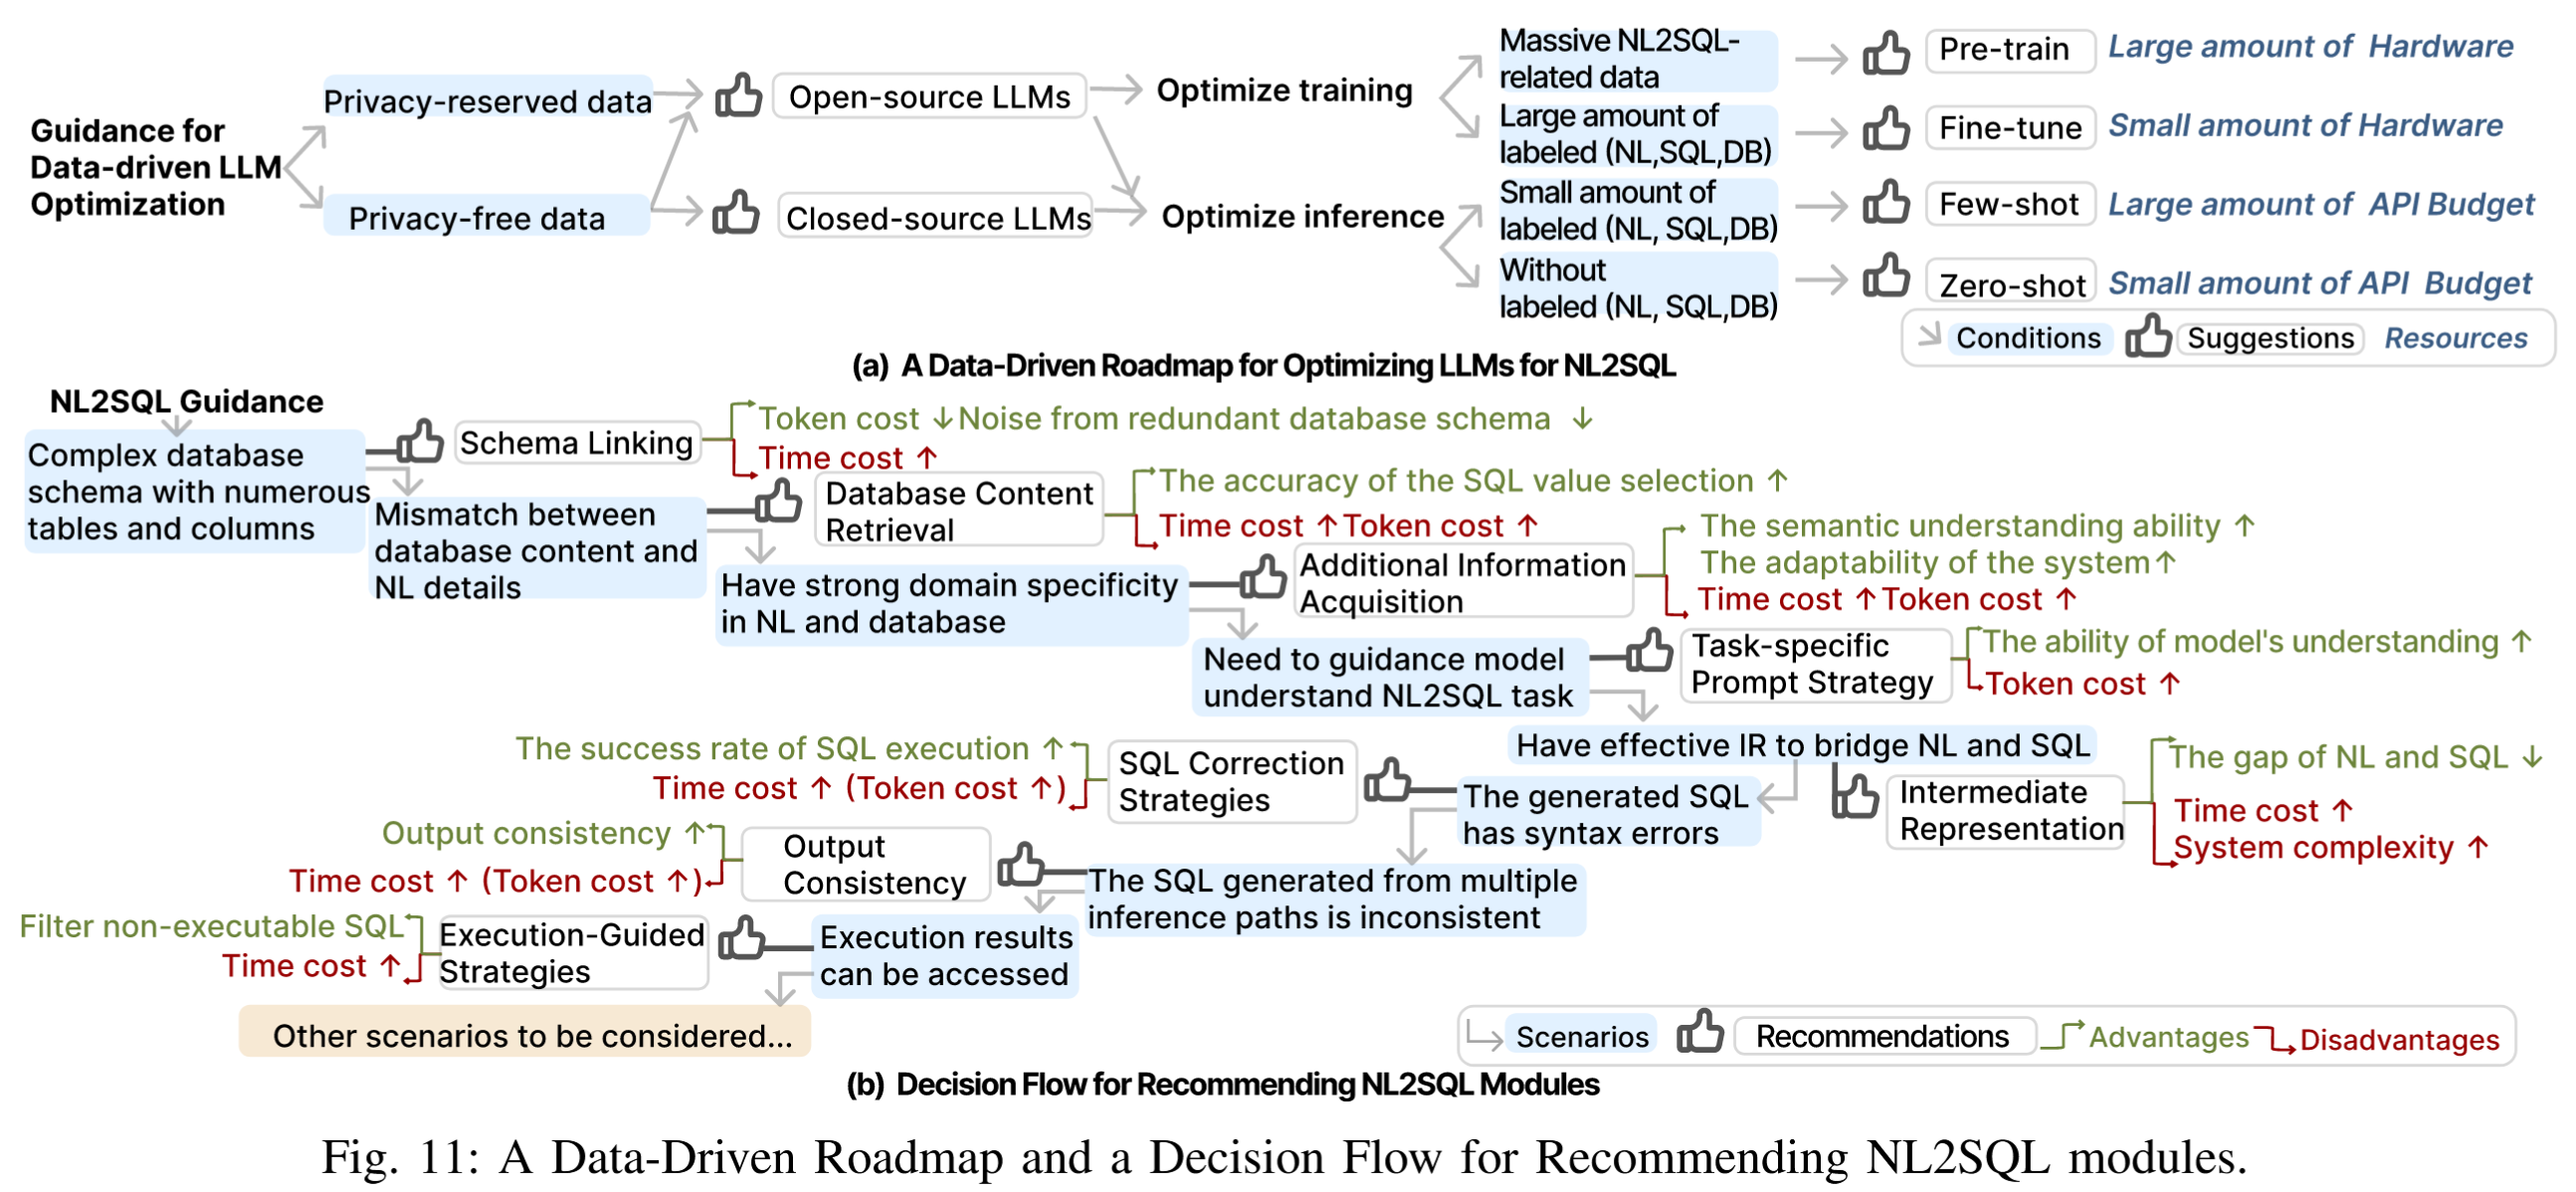
\includegraphics[width=\linewidth]{assets/roadmap.png}
    \end{figure}
\end{frame}

%------------------------------------------------

\begin{frame}{Open Problems}
\textbf{The open NL2SQL problems: }
\begin{itemize}
    \item Database retrieval: find relevant databases to access.
    \item Handling heterogeneous schemas:
    \item Answer aggregation:
    \item Domain Adaption:
    \item Scalability and efficiency:
\end{itemize}
\textbf{Developing cost-effective NL2SQL methods}:

\textbf{Make NL2SQL solutions trustworthy}:
\begin{itemize}
    \item Interpreting NL2SQL solutions:
    \item NL2SQL debugging tools:
    \item Interactive NL2SQL Tools:
\end{itemize}

\end{frame}

%------------------------------------------------

\begin{frame}
    \Huge{\centerline{\textbf{The End}}}
\end{frame}

\end{document}